\documentclass[titlepage,11pt]{article}

\usepackage{amsmath, amssymb}
\usepackage{float}
\usepackage{gensymb}
\usepackage[pdftex]{graphicx}
\usepackage[margin=1in]{geometry}
\usepackage{ragged2e}
\usepackage{setspace}
\usepackage{cleveref}
\usepackage{siunitx}% si units
\usepackage{wrapfig}
\usepackage[utf8]{inputenc} % Required for inputting international characters
\usepackage[T1]{fontenc} % Output font encoding for international characters
\usepackage{mathpazo} % Palatino font
\usepackage{xcolor}
\usepackage[sort&compress,numbers,super]{natbib}
\usepackage{caption}
\usepackage{subcaption}

\newcommand{\figfile}{C:/Users/Hayden/Documents/Patey_Lab/ThesisCodeBase/Manuscript_1.0/figures}
\newcommand{\HOS}{{\color{red}HOS}}
\newcommand{\Ham}{\widehat{\mathcal{H}}}

\begin{document}
\begin{titlepage} % Suppresses displaying the page number on the title page and the subsequent page counts as page 1
	\newcommand{\HRule}{\rule{\linewidth}{0.5mm}} % Defines a new command for horizontal lines, change thickness here
	
	\center % Centre everything on the page
	\begin{figure*}
		\centering
		
\includegraphics[width=\textwidth]{figures/UBC_Chemlogo.eps}
	\end{figure*}
	
	
	%------------------------------------------------
	%	Headings
	%------------------------------------------------
	
	\textsc{\LARGE Supplementary Information}\\[1.5cm] % Main heading such as the name of your university/college
	
	
	%------------------------------------------------
	%	Title
	%------------------------------------------------
	
	\HRule\\[0.4cm]
	
	{\huge\bfseries Exploration of Crystal Nucleation Phenomena Through Molecular Simulation}\\[0.4cm] % Title of your document
	
	\HRule\\[1.5cm]
	
	%------------------------------------------------
	%	Author(s)
	%------------------------------------------------
	
	\begin{minipage}{0.4\textwidth}
		\begin{flushleft}
			\large
			\textit{Author}\\
			Hayden \textsc{Scheiber} % Your name
		\end{flushleft}
	\end{minipage}
	~
	\begin{minipage}{0.4\textwidth}
		\begin{flushright}
			\large
			\textit{Supervisor}\\
			Dr. Gren \textsc{Patey} % Supervisor's name
		\end{flushright}
	\end{minipage}\\
	
	\vspace{1cm}
	
	\begin{minipage}{0.4\textwidth}
		\begin{flushleft}
			\large
			\textit{Chair}\\
			Dr. Geoffrey \textsc{Herring} % Chair
		\end{flushleft}
	\end{minipage}
	~
	\begin{minipage}{0.4\textwidth}
		\begin{flushright}
			\large
			\textit{Committee}\\
			Dr. Yan \textsc{Wang}\\ % Committee
			Dr. Mark \textsc{Thachuk}\\ % Committee
			Dr. Keng \textsc{Chou} % Committee
		\end{flushright}
	\end{minipage}
	
	%------------------------------------------------
	%	Date
	%------------------------------------------------
	
	\vfill\vfill\vfill % Position the date 3/4 down the remaining page
	
	{\large
		\begin{table}[H]
			\centering
			\begin{tabular}{lll}
				\textbf{Date} & \textbf{Time} & \textbf{Location} \\
				April 29$^{\text{th}}$, 2019 & 9:00 AM & CHEM D317
			\end{tabular}
		\end{table}
	}
	%------------------------------------------------
	%	Logo
	%------------------------------------------------
	
	%\vfill\vfill
	%\includegraphics[width=0.2\textwidth]{placeholder.jpg}\\[1cm] % Include a department/university logo - this will require the graphicx package
	
	%----------------------------------------------------------------------------------------
	
	\vfill % Push the date up 1/4 of the remaining page
	
\end{titlepage}

%----------------------------------------------------------------------------------------
\justifying
\doublespacing

\section{Introduction}
%
\begin{figure}
	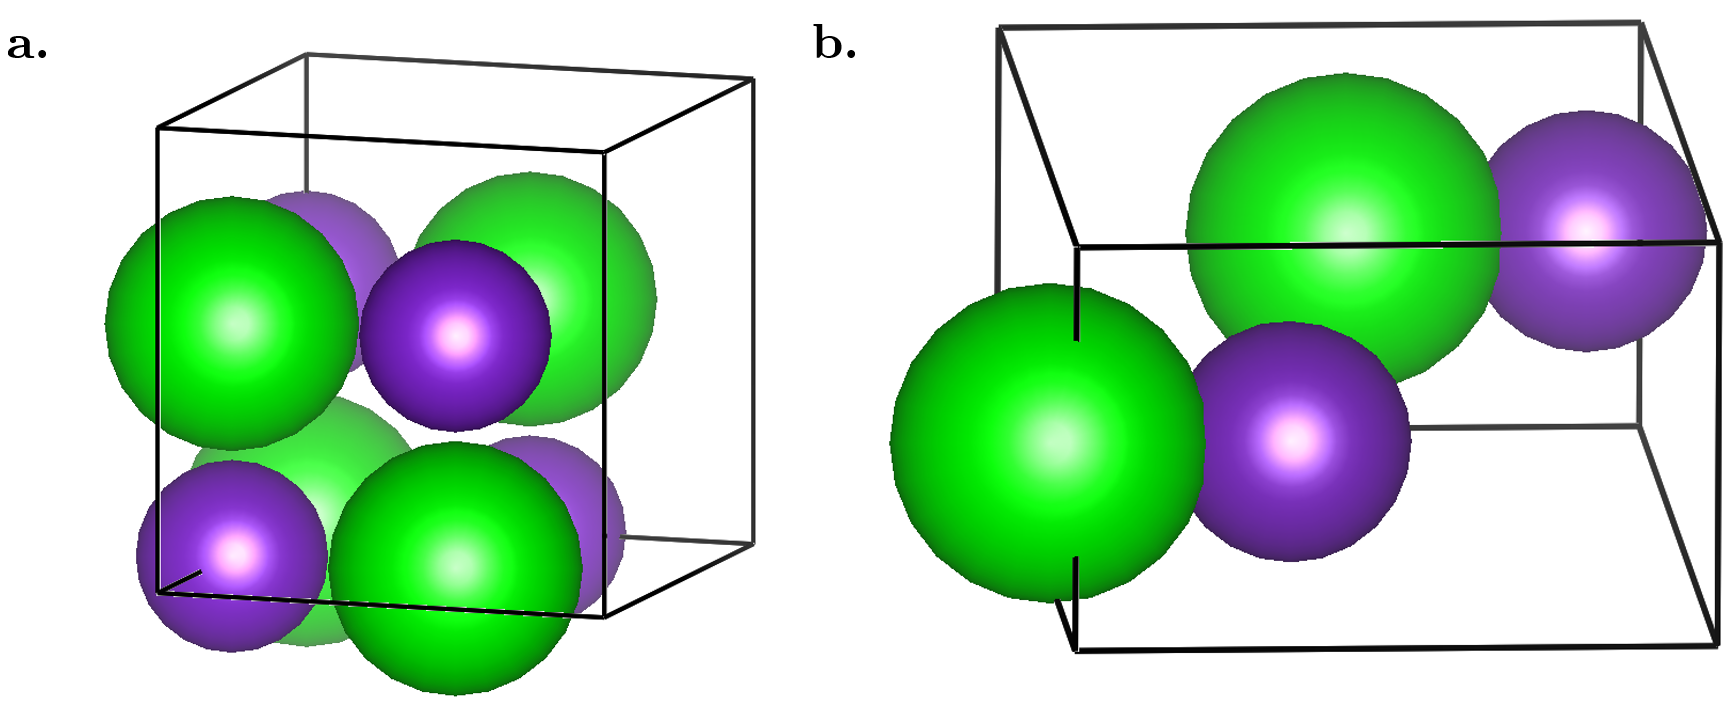
\includegraphics[width=\textwidth]{figures/Wurtzite_Rocksalt.png}
	\caption{\label{fig:structures} \textbf{a)} The rocksalt unit cell. \textbf{b)} The wurtzite unit cell.}
\end{figure}
%
		
% MODELS
\section{Models}

There are two main approaches used to calculate the experimental lattice energy. The first approach is to construct a theoretical model that encapsulates as many contributions as possible to the lattice energy, and then to fit the parameters to various data points. The first of these models, and probably the least accurate, is the Born–Land\'{e} equation from 1918,~\cite{born1918absolute}
\begin{align}
E_{Lattice} = \frac { N _ { A } M Z ^ { + } Z ^ { - } e ^ { 2 } } { 4 \pi \epsilon _ { 0 } r _ { 0 } } \left( 1 - \frac { 1 } { n } \right).
\label{eq:BornLande}
\end{align}
Here $N_{A}$ is Avagadro's number; $M$ is the Madelung constant of the crystal structure; $Z^{+}$ and $Z^{-}$ are the ion valencies; $e$ is the elementary charge; $r_{0}$ is the experimentally determined shortest distance between oppositely charged ions; $\epsilon _ { 0 }$ is the permittivity of free space; and $n$ is the Born exponent which is usually an integer between 5 and 12, obtained from experimental measurements of salt compressibilities. The equation assumes a repulsive interaction between ions proportional to $r^{-n}$, and hence misses the more realistic exponential decay from Pauli repulsion. Furthermore, any dispersion interaction, charge penetration, charge transfer interactions, and zero-point energy are entirely neglected. 

An improvement over the Born-Land\'{e} equation is the Born-Mayer equation,~\cite{Born1932,Huggins1937,Huggins1947}
\begin{align}
E_{Lattice} =  \frac { N _ { A } M Z ^ { + } Z ^ { - } e ^ { 2 } } { 4 \pi \epsilon _ { 0 } r _ { 0 } } \left( 1 - \frac { \rho } { r _ { 0 } } \right).
\label{eq:BornMayer}
\end{align}
This equation is derived by assuming an interionic repulsive term proportional to $e^{-\rho/r_{0}}$, where $\rho$ is a parameter related to the compressibility of the crystal that is, in principle, derivable from experiment (approximately $\SI{0.03}{\nano\meter}$ works well for lithium halides). The exponential form for the repulsion energy was originally derived via first-order perturbation theory for a pair of helium atoms by Slater in 1928,~\cite{Slater1928} his argument hinging on a series of approximations including spherical symmetry of electron density.~\cite{Buckingham1938} Lattice energies calculated via the Born-Mayer equation are sometimes cited as ``calculated experimental lattice energies'',~\cite{book:CRC} though they are only approximate and ignore a multitude of small --- but difficult to quantify --- contributions to the true lattice energy. Other attempts have been made to improve upon these equations,~\cite{Ladd1959} but all continue to remain as approximations.



The only fully experimental lattice energies, which are used for comparison in this report, are those calculated (indirectly) through the Born-Haber cycle.~\cite{book:CRC,Jenkins2005} The Born-Haber cycle utilizes Hess's law to calculate the lattice enthalpy in a roundabout way. This method requires summing together the following directly measurable quantities: the enthalpy of ionization for the cation; the electron affinity for the anion; the dissociation enthalpy of any species whose standard state is molecular; sublimation enthalpy for any species whose standard state is not gaseous; and the heat of formation for the salt in question. If one neglects the PV term of the salt enthalpy, the difference in \textit{energy} between the salt and the ionic gas can then be calculated, assuming the ionic gas is ideal at constant pressure and temperature, as
\begin{align}
\Delta H =  \Delta E + \Delta n R T
\label{eq:enthalpy}
\end{align}
where $\Delta n$ is change in the moles of gas per mole of crystal produced ($-2$ for a lithium halide salt). It should be noted that the assumption of ideality is particularly poor in this case considering the strong electrostatic forces at play. However, introducing a more accurate equation of state for the ionic gas is nontrivial, and will inevitably vary between species. The $\Delta E$ of equation~\ref{eq:enthalpy} is \textit{not} the lattice energy, because it does not take into account finite temperature effects nor the zero-point vibrational energy. For a generalized salt made of monatomic ions,
\begin{align}
a A^{q+}_{(g)} + b B^{p-}_{(g)} \rightarrow A_{a}B_{b},
\end{align}
these effects can be approximated by~\cite{Jenkins2005}
\begin{align}
\Delta E = E _ { Lattice } + E _ { Vib } - \left[ a \left( \frac { 3 }{ 2 } \right) + b \left( \frac{ 3 } { 2 } \right) \right] R T .
\label{eq:energyeffects}
\end{align}
The first term on the right hand side is the lattice energy, the second term accounts for the total vibrational energy of the crystal, while the third term takes into account the classical energy associated with translation in a gas. Classical rotational energy is zero in the case of monatomic ions. 

An approximation to the vibrational energy is derived from either the Debye or Einstein models for a crystal in the high temperature regime, where $E_{Vib} \approx 3(a + b) R T$. Note that light salts such as LiF are not expected to exist in the high temperature vibrational regime under ambient conditions, so this approximation overshoots the vibrational energy of such species. In addition, the classical approximation does not take into account the zero-point vibrational energy, which is species and structure dependent but not expected to be greater than approximately $\SI{10}{\kilo\joule\per\mole}$ for ionic salts.~\cite{froyen1984} Overall, the typical method used to calculate the lattice energy of non-molecular salts through the Born-Haber cycle is
\begin{align}
E_{Lattice} =\Delta H - \left[ a \left( \frac { 3 } { 2 } - 2 \right) + b \left( \frac { 3 } { 2 } - 2 \right) \right] R T.
\end{align}
This method relies on a wide range of experimental data with a range of uncertainties and potential systematic errors, such as lattice defects in the crystalline phase and the assumption of ideal gas behavior in the ionic gas. In addition, the approximations used in calculating $E_{Lattice}$ from $\Delta E$ add further uncertainty to the experimental lattice energies. It appears that no proper error analysis has been done for lithium halide lattice energies calculated using the Born-Haber cycle, and no uncertainties are reported~\cite{book:CRC}. With this in mind, the reported experimental lattice energies are clearly only approximate, with no reported error.

In light of the above situation, we decided to improve the experimental lattice energy calculations for lithium halides by delving back into the original sources for the thermochemical properties needed. The lattice enthalpy for any LiX salt at standard pressure and temperature ($\SI{298}{\kelvin}$) is calculated as
\begin{align}
 \Delta H^{\circ}_{Lattice} = \Delta H^{\circ}_{f} (\text{LiX}_{(s)}) - \Delta H_{f}^{\circ} (\text{Li}_{(g)}) - \Delta H^{\circ}_{f} (\text{X}_{(g)}) - E_{i} (\text{Li}) + E_{ea} (\text{X})
\end{align}
where $\Delta H^{\circ}_{f} (\text{LiX}_{(s)})$ is the standard enthalpy of formation for the LiX salt, $\Delta H_{f}^{\circ} (\text{Li}_{(g)})$ is the standard enthalpy of formation of gaseous lithium (equal to the enthalpy of sublimation), $\Delta H^{\circ}_{f} (\text{X}_{(g)})$ is the enthalpy of formation for the halide atom, $E_{i} (\text{Li})$ is the lithium first ionization energy, and $E_{ea} (\text{X})$ is the electron affinity of the halide. Summation of all of these quantities results in the lattice enthalpy, which for lithium halides can be separated into the following contributions
\begin{align}
\Delta H^{\circ}_{Lattice} &= H^{\circ}(\text{LiX}) - H^{\circ} (\text{Li}^{+} + \text{X}^{-})\\
&= \big( U_{Crys} + E_{ZP,Crys} + E_{Vib,Crys} + PV_{Crys} \big) - \big( U_{Ions} + E_{Trans} + PV_{Ions} \big).
\end{align}
Here we have broken up the enthalpy of the crystal into the internal potential energy $U_{Crys}$, the zero point vibrational energy $E_{ZP,Crys}$, the thermal contribution to vibrational energy $E_{Vib,Crys}$, and a $PV$ term. The enthalpy of the ions is similarly broken down into an internal potential energy term $U_{Ions}$, the thermal translation energy of the ions $E_{Trans}$, and a $PV$ term. Notice that there is no rotational energy for a system of monatomic ions. The definition of lattice energy used here is $E_{Lattice} \equiv U_{Crys} - U_{Ions}$, hence
\begin{align}
\Delta H^{\circ}_{Lattice} = E_{Lattice} + E_{ZP,Crys} + E_{Vib,Crys} + PV_{Crys} - E_{Trans} - PV_{Ions}.
\end{align}
No approximations have been made up to this point. In the CRC handbook,~\cite{book:CRC} the vibrational energy of the crystal is approximated as $3nRT$, the zero point vibrational energy is ignored, the $PV_{Crys}$ term is ignored, the translational energy of the ions is approximated by the high temperature limit of $\frac{3}{2}n R T$, and the $PV_{Ions}$ term is assumed equal to $n R T$ (an ideal gas). It turns out that all of these assumptions are more-or-less valid (to within $\approx \SI{1}{\kilo\joule\per\mole}$), except for two: ignoring the vibrational zero-point energy, and the high-temperature assumption of crystal vibrational energy.

It is possible to derive a more accurate lattice energy for the lithium halides from already existing thermodynamic data. Measurements enthalpies of formation for LiF and LiCl have been made down to $\SI{100}{\kelvin}$ with extrapolations to $\SI{0}{\kelvin}$.~\cite{chase1998nist} Uncertainties in these are measurements are reported. Similar measurements have been made for the enthalpies of formation for $Li_{(g)}$ and all the atomic halides in their gas phase.~\cite{chase1998nist,cox1984codata} The lattice enthalpy at $\SI{0}{\kelvin}$ is just
\begin{align}
\Delta H_{Lattice} (\SI{0}{\kelvin}) = E_{Lattice} + E_{ZP,Crys}.
\end{align}
An important reported thermodynamic quantity is 
\begin{align}
H^{\circ} (\text{LiX}) - H (\text{LiX}, \SI{0}{\kelvin}) = E_{vib}(\text{LiX}) + PV (\text{LiX},\SI{298}{\kelvin}) - PV (\text{LiX},\SI{0}{\kelvin}) \approx E_{vib}(\text{LiX})
\end{align}
the approximation here is almost exact, as the change in volume of a crystal between $\SI{0}{\kelvin}$ and $\SI{298}{\kelvin}$ is extremely small.



% Basis sets
\section{Basis sets}

One problem commonly associated with Gaussian basis sets is their poor transferability from molecular to periodic systems. Due to the compacted nature of periodic systems, ab initio calculations generally require specially optimized Gaussian basis sets without any diffuse basis functions, as these generate unnecessary basis function overlap leading to extremely high computation times and quasi-linear dependence between orbital functions (an artifact of finite computational precision) which can result in serious convergence problems.

% KOHN SHAM DFT
\section{HF and DFT Details}

In atomic units, the equation for the Kohn-Sham Hamiltonian is
\begin{equation}
\Ham_{KS} = -\frac{1}{2} \nabla^{2} + V_{ext}(\vec{r}) + \int \frac{\rho(\vec{r}^{\prime})}{|\vec{r} - \vec{r}^{\prime}|}d\vec{r}^{\prime} + V_{XC}[n(\vec{r})]
\end{equation}
where
\begin{equation}
\rho(\vec{r}) = \sum_{i=1}^{N} \psi_{i}^{*}(\vec{r}) \psi_{i}(\vec{r})
\end{equation}
is the electron density, $V_{ext}(\vec{r})$ is the external Coulombic potential created by the nuclei, $\psi_{i}(\vec{r})$ is the $i$-th occupied KS orbital, and $V_{XC}[n(\vec{r})]$ is the XC functional.

% HF and DFT Details

Although the CRYSTAL17 software offers an option for post-HF ab initio calculations, such calculations require a high quality correlation-consistent condensed phase basis set which, to our knowledge, does not currently exist for the lithium halides. In light of this, all of our ab initio calculations were done using Kohn Sham DFT and/or pure HF.

For all ab initio calculations performed here --- except those used to compare basis set effects --- we adopted a recently created, triple-zeta quality solid-state basis set known as pob-TZVP,~\cite{Peintinger2013,Laun2018} the acronym means: Peintinger-Oliveira-Bredow (the authors) Triple-Zeta Valence with Polarization functions. This basis set is available for all elements used in our study, and was optimized for the solid state through Kohn-Sham DFT calculations with a modified Perdew-Wang (PW) hybrid exchange-correlation (XC) functional called PW1PW.~\cite{PW1PW} The training set used to optimize the basis set parameters included lithium halide salts in the rocksalt structure,~\cite{Peintinger2013} and hence we did not need to further optimize the basis set for our uses.

For the calculation of lone ion energies ($E_{Ions}$ in equation~\ref{eq:Ions}), the pob-TZVP basis set was not a good choice due to the lack of diffuse basis functions and optimization to a crystalline environment. Lone anions naturally extend their electron density far into space in all directions, so require diffuse outer basis functions to properly capture this phenomenon. For the energy calculation of reference lone ions, we used the triple-zeta quality molecular basis set upon which pob-TZVP is derived, called def2-TZVP,~\cite{Rappoport2010,Peintinger2013} which stands for ``default version 2 - Triple Zeta Valence with added Polarizable functions''. We also augmented the basis set with the optional diffuse functions (D) in the outer orbitals, hence we will refer to the ion basis set as def2-TZVPD. As an indication of the importance of basis set in lattice energy calculation, figure~\ref{fig:basis_set} shows the difference between (fully optimized) rocksalt and wurtzite lattice energies for three basis sets. Only the pob-TZVP properly predicts the rocksalt crystal structure for all four lithium halides. In all cases, the def2-TZVP basis set was used to calculate the energy of the lone ions. The 7-311G basis set is a collection of medium quality crystalline basis sets; see refs. \citenum{ojamae1994structural} (Li), \citenum{nada1993ab} (F), \citenum{apra1993structural} (Cl), \citenum{doll1998ground} (Br and I). The STO-3G (Slater Type Orbital - 3 Gaussians) basis sets are minimum quality molecular basis sets; see refs \citenum{hehre1969program} (Li and F), \citenum{hehre1970r} (Cl), \citenum{pietro1980molecular} (Br), \citenum{pietro1981molecular} (I). Two different exchange-correlation functionals were tested: PBE~\cite{Perdew1996} and PW1PW.~\cite{PW1PW} Dispersion corrections are not included here.

In our case pure restricted Hartree-Fock calculations were used as an upper bound on the true lattice energy. The HF method computes exact exchange energy, but does not compute any correlation energy, by definition. Since correlation effects are expected to be much greater in the solid phase than in single ions, the HF method predicts lattice energies that are less negative than the true value.


In principle, the Coulomb and exchange series summations in infinite crystals involve a sum over all unit cells in the lattice. This series involves the calculation of overlap integrals between a particular atomic orbital and each of the other infinitely many atomic orbitals in the lattice. This overlap, of course, quickly decays for increasingly distant unit cells. To approximate this infinite series, the CRYSTAL17 software package demands the selection of five tolerances which define when certain overlap integrals between atomic orbitals are discarded or approximated.~\cite{Crystal17Manual} For all of our calculations, we defined the following tolerances: $\SI{e-8}{E_{H}}$ for the overlap threshold of Coulomb integrals; $\SI{e-8}{E_{H}}$ for the penetration threshold of Coulomb integrals; $\SI{e-8}{E_{H}}$ for the overlap threshold of HF exchange integrals; $\SI{e-8}{E_{H}}$ for the threshold of the pseudo-overlap for the exchange series integrals; and $\SI{e-16}{E_{H}}$ for the threshold of the second pseudo-overlap for the exchange series integrals.

For ab initio geometry optimization calculations, optimization was performed with respect to both the lattice parameters of the unit cell, and the fractional coordinates of the atoms themselves. The full symmetry of the space group was held fixed as the only constraint. For any geometry optimization calculation, a set of convergence criteria must be defined which signals the completion of the geometry optimization process. In CRYSTAL17, five convergence criteria must be fulfilled. The first criterion is the maximum change in energy between optimization steps. For our calculations, this was set to $\SI{e-11}{E_{H}}$ . The second criterion is the maximum root-mean-squared of the gradient with respect to the change in atomic positions or lattice vectors. This threshold was set to $\SI{3e-5}{E_{H} \per a_{0}}$. The third criterion is the largest component of the gradient, which was set to $\SI{4.5e-5}{E_{H} \per a_{0}}$. The fourth criterion is the root-mean-squared of the estimated displacements, which was set to $\SI{1.2e-4}{a_{0}}$. Finally, the fifth criterion is absolute value of the maximum estimated displacement, which was set to $\SI{1.8e-4}{a_{0}}$. All of these thresholds were set very tight in order to allow for robust vibrational analysis calculations later on.

In some cases, calculations had problems with SCF convergence. In order to circumvent this issue, we adopted the use of a few convergence accelerating techniques. Typically, our calculations utilized the Direct Inversion of Invariant Subspace (DIIS)~\cite{pulay1980convergence,pulay1982improved} technique to accelerate convergence. When this approach failed, we used the Fock-mixing technique, wherein each iteration of the Fock or Kohn-Sham matrix is updated with a fraction of the previous matrix. This helps to hinder oscillations. When necessary, the Fock mixing fraction was set to 40\%. In addition to Fock mixing, the the eigenvalue level shifting technique was occasionally used for serious convergence problems. This technique shifts the diagonal elements of the Fock or Kohn-Sham matrix of only the unoccupied orbitals by an input amount. The shift of 0.3 - 1.0 $E_{H}$ was typically sufficient for improving convergence. Note that this technique does not appreciably affect the resulting total energy when utilized in comparison tests.

% Basis set superposition error
\section{Basis Set Superposition Error: Counterpoise Method}

In the CP method, the energy of a lone atom or ion $i$ is first calculated using the atom-centered basis set of interest $E_{i}$. Next, all basis functions of the complete system are reintroduced without their corresponding atomic nuclei or electrons, centered on their normal sites. These ``ghost atoms'' work to expand the basis set of the lone atom/ion. The energy is recalculated with this expanded basis set resulting in a new energy $E_{i,Expanded}$, from which $E_{i}$ is subtracted. This process is repeated for each atom in the system of interest. For periodic systems, this is repeated up to a specified cutoff. The total BSSE error of a unit cell is estimated as
\begin{align}
E_{CP} = \sum_{i=1}^{N} E_{i,Expanded} - E_{i},
\end{align}
where the sum is over all atoms in the unit cell. The CP method gives a reasonable approximation to the BSSE caused by an incomplete basis set. Since our atomic calculations were done using the def2-TZVPD basis set, we used this for our CP calculations. Table~\ref{tab:BSSE} lists the resulting CP corrections for all lithium halides in both rocksalt and wurtzite configurations at their equilibrium geometries, using the PBE XC functional.


Other exchange-correlation functionals were tested as well, with similarly negligible corrections. These results are a good indication that our chosen atomic basis set is near the basis set limit. Note that it is unusual to obtain a positive value for the CP correction, as that would imply the energy was raised upon expansion of the basis set. This is possible when the original basis set is very near to the basis set limit, and addition of extra basis functions places the calculation into a self-consistent field cycle that is not the global minimum of energy. Since the size of the corrections are so small, all further calculations neglect these BSSE estimates.

% DISPERSION
\section{Dispersion}

In bulk systems, the exchange interaction acts as a repulsive force in Fermions and an attractive force in Bosons, but is not considered a true physical force due to the lack of a force-carrier particle. Rather, the exchange interaction arises naturally and unavoidably from the symmetrization conditions of identical particles that are fundamental to quantum mechanics. The exchange interaction is accounted for in the Hartree-Fock method by antisymmetrization of the all-electron wavefunction $\Psi \left( \mathbf { x } _ { 1 } , \mathbf { x } _ { 2 } , \ldots , \mathbf { x } _ { N } \right)$ with a single Slater determinant,~\cite{szabo2012modern}
%
\begin{align}
\Psi \left( \mathbf { x } _ { 1 } , \mathbf { x } _ { 2 } , \ldots , \mathbf { x } _ { N } \right) 
= \frac { 1 } { \sqrt { N ! } } 
\left| 
\begin{array} { c c c c } 
{ \chi _ { 1 } \left( \mathbf { x } _ { 1 } \right) } & { \chi _ { 2 } \left( \mathbf { x } _ { 1 } \right) } & { \cdots } & { \chi _ { N } \left( \mathbf { x } _ { 1 } \right) } \\ 
{ \chi _ { 1 } \left( \mathbf { x } _ { 2 } \right) } & { \chi _ { 2 } \left( \mathbf { x } _ { 2 } \right) } & { \cdots } & { \chi _ { N } \left( \mathbf { x } _ { 2 } \right) } \\ 
{ \vdots } & { \vdots } & { \ddots } & { \vdots } \\ 
{ \chi _ { 1 } \left( \mathbf { x } _ { N } \right) } & { \chi _ { 2 } \left( \mathbf { x } _ { N } \right) } & { \cdots } & { \chi _ { N } \left( \mathbf { x } _ { N } \right) } 
\end{array} 
\right|.
\label{eq:SlaterDet}
\end{align}
%
Here, $\mathbf { x }_{ i } = ( x, y, z , \omega)$ refers to the collection of spin and spacial coordinates for electron $i$. $N$ is the total number of electrons in the system, and $\chi_{ j } (\mathbf { x } _ { i })$ refers to the one-electron wavefunction $j$ occupied by electron $i$. By constructing a Slater determinant to represent the total wavefunction, antisymmetry is ensured between all pairs of electrons such that $\Psi \left( \mathbf { x } _ { 1 } , \ldots ,\mathbf { x } _ { i }, \ldots, \mathbf { x } _ { j }, \ldots , \mathbf { x } _ { N } \right) = - \Psi \left( \mathbf { x } _ { 1 } , \ldots ,\mathbf { x } _ { j }, \ldots, \mathbf { x } _ { i }, \ldots , \mathbf { x } _ { N } \right)$. Using the mathematical mechanism of Slater determinants requires that the quantum mechanical calculation is based on single electron wavefunctions. DFT, however, is not a wavefunction-based calculation. Instead, DFT calculations are based on functionals of \textit{electron density}, such that Slater determinants cannot be used for the calculation of exchange energies. In DFT, the exchange interaction is introduced through the exchange functional. Similarly the correlation energy is expressed through the correlation functional. Neither of these functionals have known exact forms, so DFT is not currently capable of accounting for dispersion.
	
	
	
	
	
	
In an attempt to compensate for the lack of exact dispersion in DFT, several approaches have been introduced.~\cite{grimme2016dispersion} The most advanced of which is arguably D3(BJ) dispersion,~\cite{Grimme2010,grimme2016dispersion,Becke2007,Grimme2011} which adds an additional dispersion energy to the total energy calculated from DFT as
\begin{equation}
E_{\text { total }} = E_{\text { DFT } } + E_{\text { disp } }
\end{equation}
where $E_{\text { DFT } }$ is the usual total energy of the system. In the D3(BJ) approach as implemented in CRYSTAL17,~\cite{Crystal17Manual} the dispersion energy is approximated by a sum of two-body terms as
\begin{equation}
E _ { \text { disp } } = - \sum _ { i > j } \bigg( \frac { C _ { 6 , i j } } { R _ { \text {vdW}, i j } ^ { 6 } + r _ { i j } ^ { 6 } } + \frac { C _ { 8 , i j } } { R _ { \text {vdW}, i j } ^ { 8 } + r _ { i j } ^ { 8 } }  \bigg)
\label{eq:Dispersion}
\end{equation}
where $C _ { n , i j }$ are the dispersion coefficients --- representing transient dipole-dipole and dipole-quadrupole interactions --- which are estimated from time-dependent DFT calculations of dynamical polarizabilities. These pre-calculated coefficients are then mapped to the system under consideration based on the coordination number of each atom, calculated on-the-fly. $R _ { \text {vdW}, i j }$ is the damping radius, calculated from the dispersion coefficients as well as two global XC-dependent parameters. This damping radius must be included to prevent non-physical singularities in the potential for small $r_{ij}$.~\cite{grimme2016dispersion} Three-body terms for D3(BJ) dispersion have also been developed, but in initial tests did not significantly affect the outcome of our calculations.
	
	
\section{Conclusion}

At the time of writing this report, I have used DFT calculations implemented through the CRYSTAL17 code~\cite{Crystal17} to thoroughly explore lithium halide crystalline systems in the solid state. I found that when properly optimized, modern DFT calculations can accurately predict experimental equilibrium lattice parameters (to within a few percent) and crystal structures for lithium halides. The associated equilibrium crystal lattice energies also appear to be very reasonable, although these are more difficult to compare with experiment. In the future, I will use this wealth of data to produce improved lithium halide models for non-classical nucleation research.

\singlespacing
\bibliographystyle{achemso}
\bibliography{references}
	
\end{document}